\documentclass[10pt]{exam}
\usepackage[hon]{template-for-exam}
\usepackage{tikz,multicol,cclicenses,hyperref}
\usetikzlibrary{shadings,shadows,arrows.meta,shapes.geometric}


\title{Rotational Energy}
\author{Rohrbach}
\date{\today}

\begin{document}
\maketitle


\section*{Quantities}

\renewcommand{\arraystretch}{2}

\begin{tabular}{p{9em}ccp{6.5em}}
  Concept & Linear/Translational Quantity & Angular/Rotational Quantity & \hfill ``Bridge'' \\ \hline\hline
  kinetic energy \\[1em] & units: & units:  \\\hline
  work \\[1em] & units: & units:  \\\hline
\end{tabular}

\pagebreak


\section*{Practice}

Consider a solid disc that is released from rest at the top of a ramp that is 5 meters tall. Assume that the disc does not slip and is perfectly round. How fast will the disc be going when it gets to the bottom of the ramp?

\vs[2]

\pagebreak

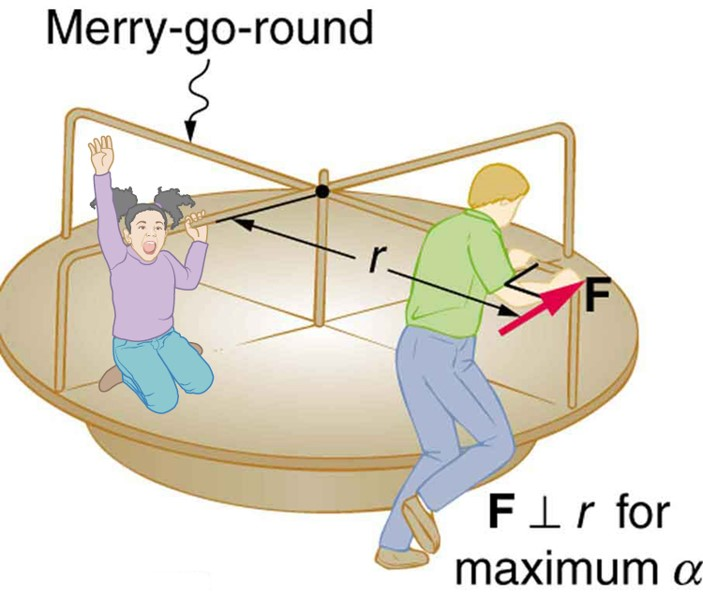
\includegraphics[width=7cm]{merrygoround.jpg}


{\footnotesize Image Credit: OpenStax \emph{College Physics}: 2nd Ed. Rice University. }

{\footnotesize License:} \cc\hspace{-1em}\ccby  {\footnotesize CC BY 4.0}

{\footnotesize Retrieved 2025-02-11 from \texttt{\href{https://openstax.org/books/college-physics-2e/pages/10-3-dynamics-of-rotational-motion-rotational-inertia}{https://openstax.org/books/college-physics-2e/}} }


\vspace{2em}
\noindent
Consider the father pushing a playground merry-go-round. The 50.0-kg merry-go-round has a 1.50 m radius.  An 18.0-kg child sits 1.25 m away from the center. Consider the merry-go-round itself to be a uniform disk with negligible friction and the child to be a particle.  If the merry-go-round rotates at 40 rpm, what is the rotational KE?



\end{document}